\documentclass[a4paper]{article}

\usepackage[T1]{fontenc}
\usepackage[utf8]{inputenc}
\usepackage[spanish]{babel}
\usepackage{etoolbox}
\usepackage{graphicx}
\usepackage{framed}
\usepackage{epstopdf}
\usepackage{enumerate}
\usepackage{amsmath}
\usepackage{amsthm}
\usepackage{amssymb}
\usepackage{amsfonts}
\usepackage{cancel}
\usepackage{tabularx}
\usepackage{tabu}
\usepackage{booktabs}
\usepackage{float}
\usepackage{array}
\usepackage{multirow}
\usepackage{verbatim}
\usepackage{tikz}
\usetikzlibrary{arrows,positioning,calc,shapes.geometric}
\graphicspath{ {images/}{Exercises/images/}{Header/} }
\providetoggle{showAnswers}
\providetoggle{eachProblemInOnePage}
\usepackage{graphicx}
\usepackage{epstopdf}
\usepackage[export]{adjustbox}
\usepackage{caption}
\usepackage{colortbl} 
\usepackage{dashrule} 
\usepackage{fancyhdr}
\usepackage[bmargin=2cm,footnotesep=1cm,tmargin=2cm]{geometry} 
\usepackage[pdftex,colorlinks,a4paper,backref,bookmarks=true,bookmarksnumbered=true,linkcolor=blue,urlcolor=blue,citecolor=blue]{hyperref}
\usepackage[section]{placeins}
\usepackage[labelsep=quad,indention=10pt]{subfig}
\usepackage[spanish,shadow,textsize=small]{todonotes}
\usepackage{wrapfig}
\usepackage{karnaugh-map}

% Código fuente
\newcommand{\code}[1]{\texttt{#1}}

% Minted
\usepackage{minted}
% Optional: Set a default style. 'manni' is a light, clean style.
% Other popular styles include 'tango', 'monokai', 'solarized-light'.
\usemintedstyle{sas}

% Cajas de respuestas
\newcommand{\overflowbox}[1]{%
    \enlargethispage{\textheight}
    \nobreak
    \noindent
    \fbox{%
        \parbox{\textwidth}{%
            \rule{0pt}{#1}%
        }%
    }%
}

% Caja sombreado
% comando \sombreado{Título}{Texto}
\definecolor{shadecolor}{rgb}{0.9,0.9,0.9}
\newcommand{\sombreado}[2]{
  \begin{shaded}
    \begin{center} \emph{\textsc{#1}} \end{center}
    \noindent #2\\
  \end{shaded}
}


% PARAMETROS CONFIGURABLES
\newcommand{\asig}{Algoritmos y Estructuras de Datos}
\newcommand{\grado}{Grado en Ingeniería Biomédica}
\newcommand{\ceu}{Universidad Politécnica de Madrid}
\newcommand{\autor}{Rodrigo García Carmona}
\newcommand{\email}{\href{mailto:rodrigo.garcia@upm.es}{rodrigo.garcia@upm.es}}
\newcommand{\titulo}{Concurrencia y sincronización - Ejercicios}

% PDF
\hypersetup{
  pdfauthor={\autor},
  pdftitle={\titulo},
  pdfsubject={\asig, \grado, \ceu}, 
  pdftoolbar=true,
  pdfmenubar=true,
  pdffitwindow=true,
  pdfnewwindow=true
}

% ENCABEZADO
\pagestyle{fancy}%
  \renewcommand{\headrulewidth}{0.1pt}
  \renewcommand{\footrulewidth}{0.1pt}
  \fancyhf{}
  \fancyhead[L]{
\includegraphics[width=8mm]{templates/ETSIT-UPM.eps}}
  \fancyhead[C]{\small{\asig}\\\small{\grado}}
  \fancyfoot[L]{}
  \fancyfoot[C]{\thepage}
  \fancyfoot[R]{}

% CONTENIDO
\begin{document}

\input{titlepage.tex}

\section{Introducción}

A continuación encontrará los enunciados de una serie de ejercicios que le servirán para practicar. Para cada ejercicio, aunque no se especifique, no deje de tener en cuenta que:

\begin{itemize}
    \item Debe considerar los casos límite o problemáticos como arrays vacíos, valores \code{null}, índices fuera de rango...
    \item El código debe ser eficiente: si es posible evitar un bucle, ahorrar vueltas dentro de un bucle o reducir el número de líneas a ejecutar, es mejor hacerlo.
    \item Lo programado debe ser legible, intentando que el código sea fácil de entender y acompañándolo de comentarios completos pero concisos.
    \item Puede organizar su código en paquetes y clases, así como reutilizar métodos ya creados. Un buen método debería caber en una única pantalla.
\end{itemize}

Además, no deje de probar su código. No se limite a ver que compila o que funciona con una entrada de datos trivial.

\section{Ejercicios}

\subsection{Lectores y escritores}

Cree un programa en el que un conjunto de hebras acceden a un único recurso compartido: un número entero (realmente, podría ser cualquier tipo de dato). Estas hebras pueden ser de uno de los siguientes dos tipos:

\begin{itemize}
    \item \textbf{Lectora:} Lee una vez el entero y lo imprime por pantalla.
    \item \textbf{Escritora:} Sustituye el entero por otro valor entero generado aleatoriamente, entre 0 y 10.000.
\end{itemize}

El número y tipo de cada hebra deberá ser configurable, ya sea mediante argumentos del método \code{main()} o mediante atributos estáticos de una clase. Su programa deberá permitir que:

\begin{itemize}
    \item Varias hebras lectoras accedan al entero al mismo tiempo.
    \item Impedir que, cuando una hebra escritora está accediendo al entero, ninguna otra hebra (de ninguno de los dos tipos) acceda al entero.
\end{itemize}

\subsection{Lectores y escritores: dos datos}

Modifique el problema anterior para que esta vez se controle el acceso a dos recursos compartidos \textbf{independientes}: dos enteros. Ahora los dos tipos de hebras serán:

\begin{itemize}
    \item \textbf{Lectora:} Lee un entero y lo imprime por pantalla, lee el otro entero y lo imprime por pantalla. El orden en el que se leen los enteros se determina al azar.
    \item \textbf{Escritora:} Sustituye uno de los dos enteros (determinado aleatoriamente) por otro valor entero generado aleatoriamente, entre 0 y 10.000.
\end{itemize}

Deberán respetarse las mismas dos condiciones que en el ejercicio anterior, pero en este caso el acceso a cada entero será controlado \textbf{de forma independiente}. Es decir, que si, por ejemplo, una hebra está modificando el primer entero, no habrá problema alguno en que otra hebra escriba (o lea) el segundo entero.

\subsection{Lectores y escritores: prioridades}

Modifique el primer problema para que todas las hebras tengan asociada una prioridad: alta, media o baja. Al igual que en aquel ejercicio, si una hebra quiere acceder al entero pero este está siendo escrito, deberá esperar. La diferencia es que ahora, cuando el entero quede libre, deberá seleccionarse a la siguiente hebra que va a poder acceder a él de la siguiente forma:

\begin{enumerate}
    \item Se elige una de las hebras de mayor prioridad.
    \item Si hay varias hebras con la prioridad más alta, se elige una de lectura.
    \item Si hay varias hebras de lectura con la prioridad más alta, se elige una de ellas al azar.
\end{enumerate}

Una vez termine el ejercicio, si se siente valiente, modifique el segundo ejercicio (el de los dos datos) para que también siga este esquema de prioridades.

\subsection{Productor y consumidor con una cola}

Se dispone de un \textit{buffer}, que es un array de 10 enteros. Cree un programa en el que haya dos tipos de hebras:

\begin{itemize}
    \item \textbf{Productoras:} Introducen un dato en el \textit{buffer}. Este dato será un entero generado aleatoriamente entre 0 y 10.000. Si el \textit{buffer} está lleno, deberán esperar a que una hebra consumidora borre uno de los datos del \textit{buffer}.
    \item \textbf{Consumidoras:} Leen un dato del \textit{buffer}, lo imprimen por pantalla y lo borran. Si el \textit{buffer} está vacío, deberán esperar a que una hebra productora introduzca un nuevo dato en el \textit{buffer}.
\end{itemize}

Como en ejercicios anteriores, su programa deberá poder lanzar un número arbitrario y configurable de hebras. Decida usted mismo la estructura de su programa y los detalles de implementación, pero tenga en cuenta que los datos introducidos en el \textit{buffer} deberán ser leídos en el orden en que se insertaron. Es decir, que se trata de una cola.

\subsection{La cena de los filósofos}

Cinco filósofos dedican su tiempo a pensar y a comer, alternativamente. Los filósofos están sentados en una mesa circular con cinco sillas. Delante de cada una de ellas hay un plato de espaguetis \href{https://canalcocina.es/receta/espaguetis-putanesca}{a la putanesca}. A la derecha de cada plato hay un tenedor. La Figura \ref{fig:filosofos} muestra esta disposición.

\begin{figure}[!htbp]
  \centering
  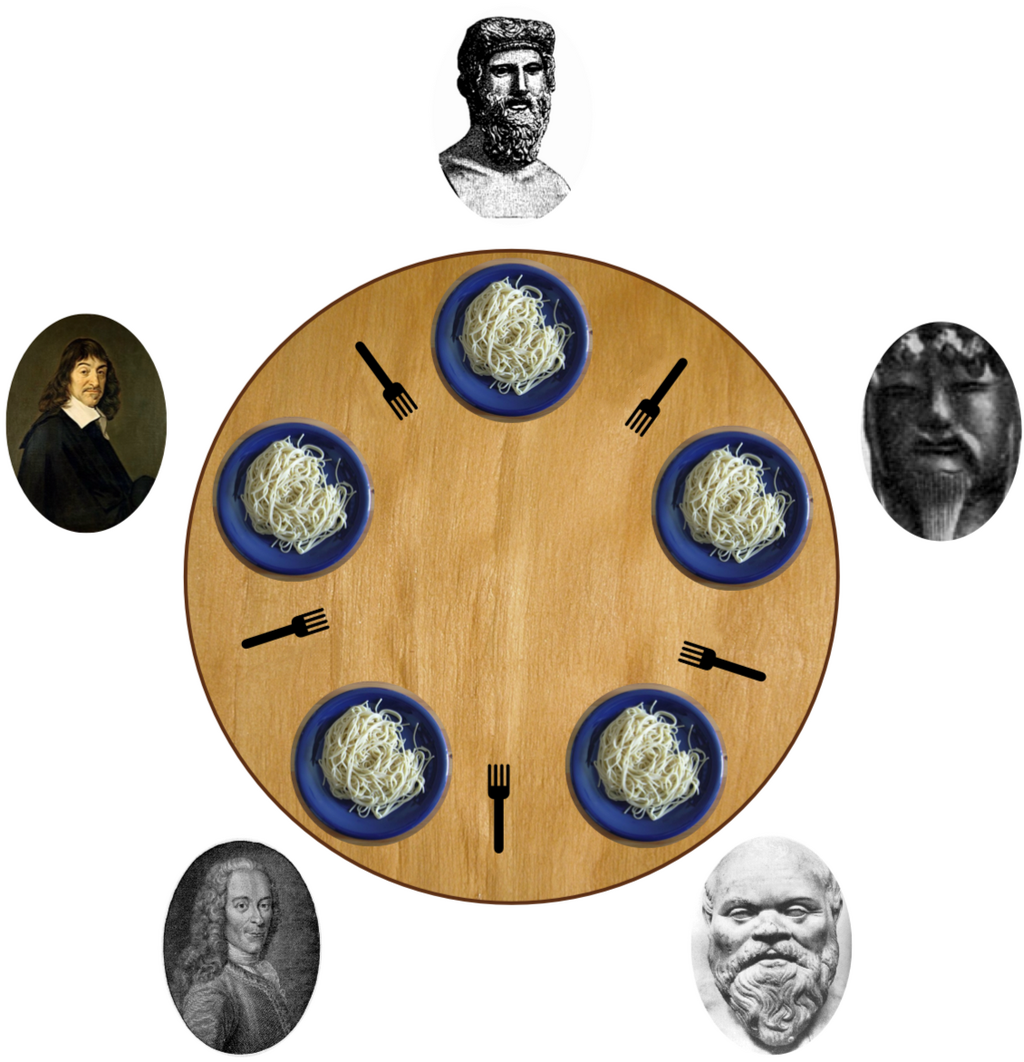
\includegraphics[width=0.6\textwidth]{files/Philosophers.png}
  \caption{La cena de los filósofos\footnotemark}
  \label{fig:filosofos}
\end{figure}
\footnotetext{\href{https://commons.wikimedia.org/w/index.php?curid=56559}{Benjamin D. Esham - CC BY-SA 3.0}}

Cuando un filósofo decide comer, toma los tenedores que tiene a su derecha y a su izquierda y, cuando tiene ambos en las manos, los utiliza para llevarse la comida a la boca. Si otro
filósofo ha cogido uno de los palillos, deberá esperar a que lo deje en la mesa.

Programe una implementación de esta cena que esté libre de interbloqueos.

\subsection{Los caníbales}

En este problema hay dos tipos de agentes: los caníbales (que comen) y el cocinero (que prepara la comida).

Los caníbales comen de una gran marmita común que contiene $n$ raciones de rico estofado de persona, pero solo un cucharón. Cuando un caníbal quiere comer, se sirve él mismo de la marmita, a menos que esté vacía. Si la marmita está vacía, el caníbal avisa al cocinero y espera a que el cocinero haya rellenado por completo la marmita. Cuando el cocinero termina, \textbf{antes de dejar comer a otro caníbal}, el caníbal que le avisó se sirve. El cocinero, por su parte, una vez ha terminado de rellenar la marmita, se sienta a esperar a que le avisen de nuevo.

Se debe desarrollar un monitor (\code{Marmita}) con dos métodos, uno que invocan los caníbales cuando quieren comer (\code{comer}), y otro que invoca el cocinero para rellenar la marmita (\code{rellenar}). El programa desarrollado debe estar libre de interbloqueos, y debe permitir que se despierte al cocinero sólo cuando la marmita esté vacía.

Decida usted mismo cuánto tiempo debe tardar el cocinero en rellenar la marmita, cada cuánto tiempo se sirve un caníbal, cuánto tiempo tarda en servirse, y cuántas veces lo hace antes de sentirse satisfecho y parar de comer. Le recomiendo que use números aleatorios para darle más gracia al asunto.

\subsection{Los tres fumadores}

En frente de un estanco se encuentran tres fumadores de dudoso aspecto. Cada fumador está continuamente (sí, continuamente) liando un cigarrillo y después fumándoselo (sí, todo el día). Para liar un cigarrillo y fumárselo, el fumador necesita tres componentes: una unidad de tabaco, un papel y una cerilla. Uno de los fumadores llega al estanco con una cantidad infinita de tabaco, otro con un número infinito de papeles y el tercero con un número infinito de cerillas. El estanquero, por su parte, tiene una cantidad infinita de los tres materiales.

Acostumbrado a la presencia de estos clientes habituales, el estanquero deja, en una mesa en la puerta del estanco, dos de los tres componentes necesarios para poder liarse y fumar un cigarro. El fumador que tiene el componente que falta coge esos dos, se lía y se fuma un cigarrillo, y avisa al estanquero cuando termina. Este pone otros dos de los tres componente en la mesa, y el ciclo se repite.

Implemente esta curiosa situación.

\subsection{Los tres fumadores solidarios}

Se da una situación idéntica a la del problema anterior, pero ahora el estanquero deja en la mesa solo uno de los tres componentes cada vez. Por tanto, para poder liarse y fumar un cigarrillo, un fumador ahora tendrá que tomar el componente que pone el estanquero y pedir a otro de los tres fumadores que le dé el componente que le falta. Como los fumadores siempre tratan bien a los suyos, los fumadores siempre acceden a compartir su componente con otro. Aunque, eso sí, solo compartirán su componente si el que lo pide ya ha cogido el componente que le ofrecía el estanquero; pedir a otro fumador está bien, pero pedir a dos es pasarse.

Implemente esta versión más humana del problema anterior.

\subsection{Delegación de Hacienda}

Hoy es un día duro en el trabajo para Andrés Trozado, funcionario en la Delegación de Hacienda. Su compañero de trabajo, Francisco Rupto, bajó a tomar ``un cafetito rápido'' hace ya más de dos horas, y aún no ha vuelto. Basándose en experiencias previas, Andrés asume que su compañero no va a volver, por lo que le va a tocar a él encargarse de las dos ventanillas de la oficina.

La oficina funciona de la siguiente manera:

\begin{itemize}
    \item Cuando un ciudadano llega a la oficina, éste espera en su ventanilla correspondiente (la 1 o la 2, dependiendo de a qué haya venido) hasta que Andrés le atiende (desbloquea). Una vez Andrés le ha atendido el ciudadano se marcha por dónde ha venido (posiblemente algo enfadado).
    \item Andrés atiende a los ciudadanos uno por uno y, cuando no quedan ciudadanos en ninguna de las dos colas, se echa una siestecita rápida, para rendir mejor. Andrés atiende en cada momento a un ciudadano de la ventanilla en la que haya más gente esperando, cambiando de ventanilla si fuera necesario. En caso de empate atiende siempre a la ventanilla 1 antes.
    \item Si mientras Andrés está durmiendo llega un ciudadano éste carraspeará, despertando (desbloqueando) al cansado funcionario con el ruido. Por tanto, un ciudadano sólo despertará a Andrés si no hay ningún otro ciudadano en la oficina.
\end{itemize}

Tanto los ciudadanos como Andrés el funcionario están modelados cada uno como una hebra.

Desarrolle un monitor que sincronice a los ciudadanos y al funcionario, según la especificación anterior, con los siguientes métodos:

\begin{itemize}
    \item \code{esperarVentanilla1()}: este método lo invoca un ciudadano cuando quiere esperar en la ventanilla 1. Cada ciudadano que quiere acceder a la ventanilla 1 lo ejecuta una vez.
    \item \code{esperarVentanilla2()}: este método lo invoca un ciudadano cuando quiere esperar en la ventanilla 2. Cada ciudadano que quiere acceder a la ventanilla 2 lo ejecuta una vez.
    \item \code{atenderCiudadano()}: este método lo ejecuta el funcionario cuando va a atender a un ciudadanos. El funcionario está ejecutando continuamente esta operación.
\end{itemize}

Tenga en cuenta que es necesario garantizar que el orden en que se atiende a los ciudadanos coincide con el orden de llegada.

\subsection{El puente de Talavera}

El Puente de Castilla la Mancha, situado en Talavera de la Reina, pasará a la historia como uno de los ejemplos más flagrantes del despilfarro por parte de los gobiernos comunitarios en España durante la década de los 2000. Cruzando el Tajo, este puente ha batido numerosos récords, entre ellos el de ser el más ancho de Europa (36 metros), incluyendo calzadas, aceras, medianas y carril bici. El Puente de Castilla la Mancha costó 90 millones de euros, por lo que, teniendo en cuenta la baja población de Talavera de la Reina, tocan a unos 1.000 € por habitante de la ciudad.

Desgraciadamente, y poco después de su construcción (Junio de 2011), uno de los cables del puente se soltó, con lo que no pudo abrirse al tráfico rodado hasta ser reparado. Afortunadamente en aquel momento había dinero para efectuar tal reparación, pero si algo así volviera a suceder, no podría darse el caso. Sin embargo, los peritos calculan que el puente podría seguir funcionando de forma limitada con un cable menos, siempre y cuando el puente no cargue más de 15.000 Kg. o 10 vehículos a la vez.

Imaginemos que sucediera tal desastre. Para evitar que el puente se colapse por completo los consejeros han recomendado al gobierno regional que contrate a un ingeniero para que diseñe un sistema para controlar el paso de vehículos. Y a ser posible de la forma lo más barata posible, que ya se han dejado mucho dinero en subcontratas de familiares y amigos.

Es su responsabilidad diseñar este sistema de seguridad, que debe impedir que el puente cargue más de 15.000 Kg. a la vez y no haya simultáneamente más de 10 vehículos atravesándolo. Implementará este sistema usando un monitor.

Este monitor contará con dos métodos. Cuando un vehículo quiera entrar en el puente ejecutará el método \code{entrarPuente()}, y cuando quiera abandonar el puente ejecutará el método \code{salirPuente()}. Los dos métodos tienen como parámetro el peso del vehículo, y el método \code{entrarPuente()} tiene además otro parámetro de tipo \code{boolean} que indica si el vehículo es una ambulancia. Esto es así porque las ambulancias tienen siempre preferencia.

La cabecera de los métodos queda, por tanto, así:

\begin{minted}[
frame=lines, % Adds a frame around the code
framesep=2mm,
% linenos % Enables line numbers
]{java}
void entrarPuente (int peso, boolean ambulancia)
void salirPuente (int peso)
\end{minted}

Un vehículo no puede recibir permiso para entrar en el puente si, dadas sus características o el estado del puente, se incumplen los requisitos de seguridad. Además, las ambulancias tienen siempre prioridad para acceder al puente respecto al resto de vehículos.

\subsection{La fábrica de LEGO}

LEGO fue fundada en el año 1932 por un carpintero Danés llamado Ole Kirk Christiansen, aunque no recibiría su nombre (que viene de la frase ``leg godt'', que significa ``jugar bien'') hasta dos años después.

En el año 1947 Christiansen decidió diversificarse y empezar a trabajar con juguetes de plástico. Uno de estos juguetes, que sería el que finalmente catapultaría a la empresa al estrellato, sus famosos bloques interconectables, comenzó su producción en el año 1949.

Sin embargo, fue Godtfred Kirk Christiansen (el hijo de Ole Kirk) quién se dio cuenta del potencial de estos bloques, y decidió patentarlos en el año 1958 y empezar a exportarlos a todo el mundo. El resto es historia, y hoy en día los modelos LEGO se encuentran entre los más codiciados juguetes, incluso por los no tan niños. Destacan líneas como LEGO Technic, y hay modelos realmente espectaculares, como el de la nave Halcón Milenario de la Guerra de las Galaxias, que cuenta con casi 5.200 piezas.

El lema de LEGO es ``sólo lo mejor es lo mejor'', por lo que en la empresa siempre intentan alcanzar las cotas de calidad más altas. Este hecho, unido a su impresionante producción (más de 1.100 bloques por segundo), hace necesaria la automatización del sistema de producción de piezas. Para ello han contratado a un joven estudiante de ingeniería: usted.

El sistema de fabricación tiene una línea para piezas rojas y otra para piezas azules. Cada línea de producción almacena las piezas producidas en una cesta distinta, con capacidad para 50 piezas cada una. Además, hay un sistema automático de gestión de pedidos, que cuenta con varios gestores de pedidos, que se encargan de extraer de cada una de las dos cestas las piezas de cada color necesarias para construir el modelo solicitado.

Tanto las líneas de producción como los gestores de pedidos están modelados como hebras, de la siguiente manera:

\begin{itemize}
    \item \code{LineaRoja}: si hay sitio en la cesta de piezas rojas, produce una pieza roja y la deposita en la cesta de piezas rojas.
    \item \code{LineaAzul}: si hay sitio en la cesta de piezas azules, produce una pieza azul y la deposita en la cesta de piezas azules.
    \item code{GestorPedidos}: extrae de ambas cestas las piezas necesarias para cumplir con el pedido.
\end{itemize}

Implemente el sistema pedido. Tenga en cuenta, que puede haber al mismo tiempo \textbf{más de un} gestor de pedidos.

\subsection{El aire acondicionado roto}

En Aranjuez se encuentra uno de los museos más curiosos de la Comunidad de Madrid: el Museo de Falúas Reales. Por si se lo pregunta, las falúas reales eran pequeñas embarcaciones fluviales utilizadas por los reyes para distraerse cuando el aburrimiento se apoderaba de ellos. Similares a góndolas, estas barcas surcaban el Tajo (de ahí que el museo esté en Aranjuez), el estanque de El Retiro o la laguna de Ontígola. La Figura \ref{fig:falua} muestra una de las más llamativas del museo.

\begin{figure}[!htbp]
  \centering
  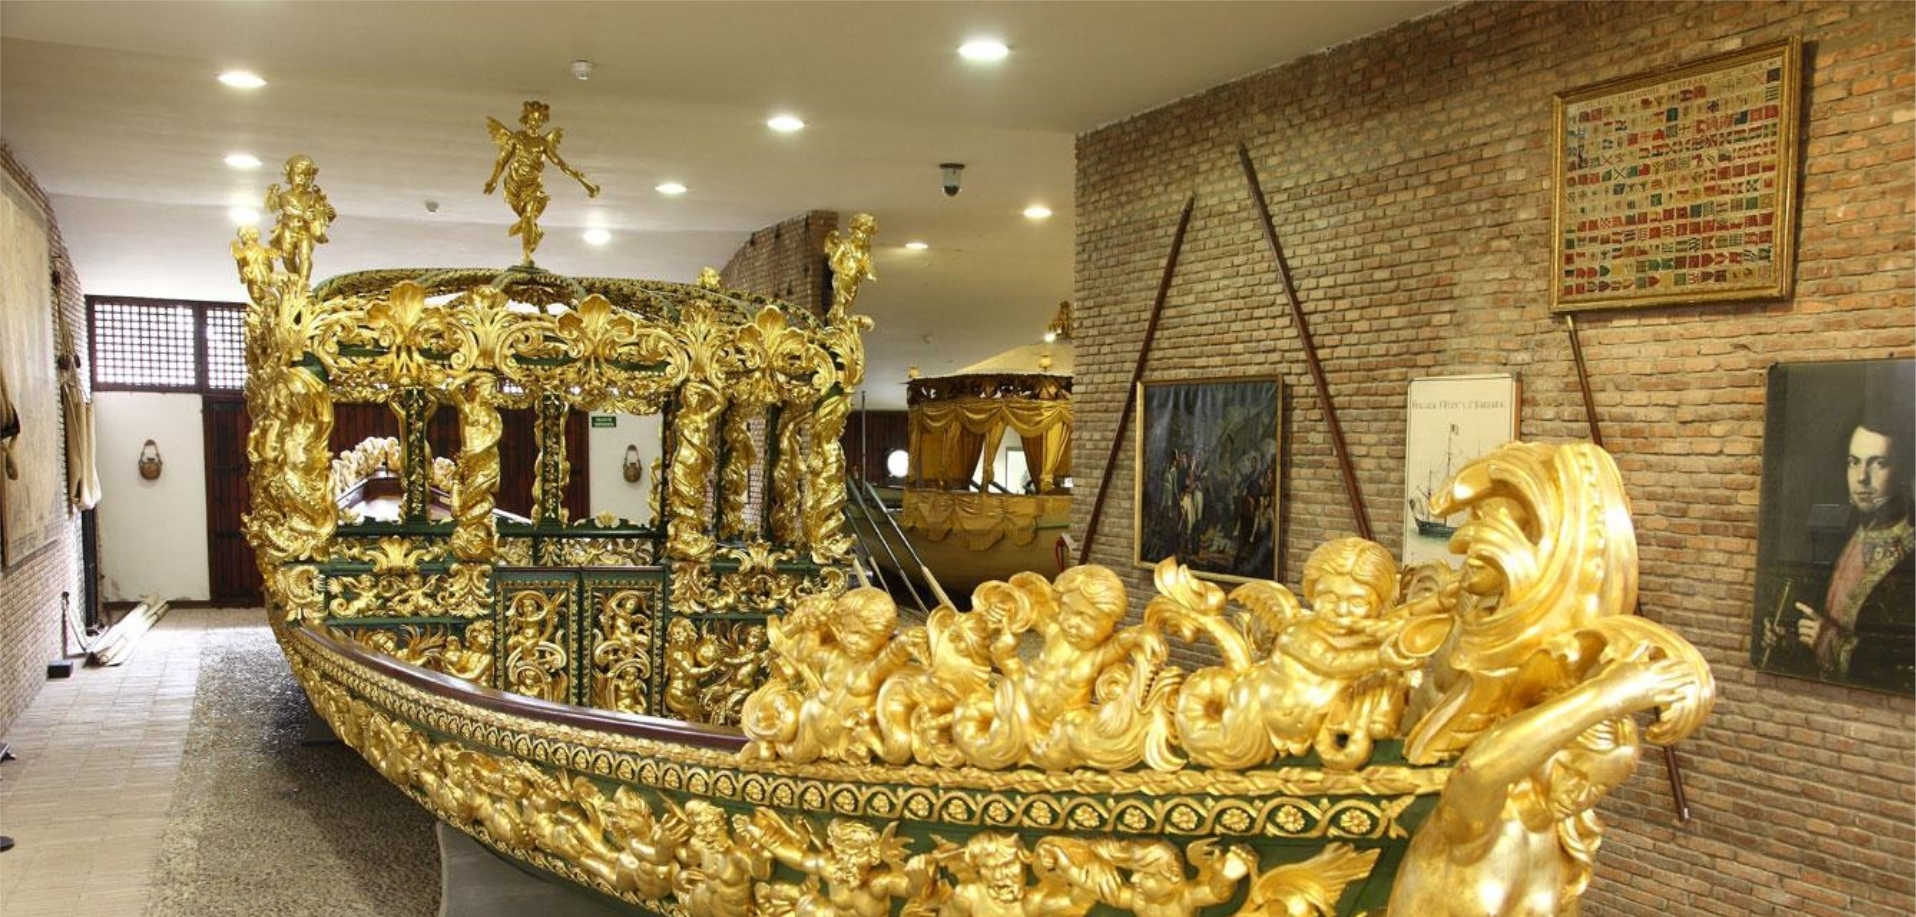
\includegraphics[width=0.8\textwidth]{files/GondolaCarlosII.png}
  \caption{Góndola napolitana de Carlos II\footnotemark}
  \label{fig:falua}
\end{figure}
\footnotetext{\href{https://www.patrimonionacional.es/colecciones-reales/faluas/gondola-napolitana-de-carlos-ii}{Colecciones del Patrimonio Nacional}}

Supongamos que este museo, por falta de presupuesto, se ve obligado a apagar su aire acondicionado (esto ya le sucedió \href{https://www.elconfidencial.com/cultura/2019-07-02/35-grados-sin-aire-acondicionado-museo-traje-obligado-cerrar-sus-puertas_2102470/}{al museo del traje}). Ante esta tesitura, la organización del Museo de Falúas ha decidido que, cuando la temperatura suba por encima de cierto umbral, deberá reducirse el número de asistentes admitidos.

Deberá implementar un sistema que controle la temperatura y el número de personas que acceden a este museo. En condiciones normales, se permite el acceso a 50 personas en la sala, pero, si la temperatura sube por encima de 30\textdegree C, se limita el número de personas a 35. Si cuando se detecta este suceso el número de personas en la sala es mayor que 35, no es necesario desalojarlas, simplemente se espera a que abandonen el museo cuando lo consideren oportuno.

En lo que a la entrada al museo respecta, hay una cola ordenada pero, por respeto a los mayores, si una persona jubilada intenta entrar, tendrá prioridad frente al resto de personas que estén esperando.

Cada persona se representa mediante una hebra. Además, hay otra hebra que mide periódicamente la temperatura del museo y actualiza el valor de esta temperatura en el sistema.

Deberá desarrollar un monitor (\code{GestorMuseo}) que sincronice a las hebras que representan personas y a la hebra que mide la temperatura, de acuerdo con las especificaciones anteriores. El monitor debe proporcionar los siguientes métodos:

\begin{minted}[
frame=lines, % Adds a frame around the code
framesep=2mm,
% linenos % Enables line numbers
]{java}
// Se invoca cuando una persona quiere entrar en el museo.
void entrarSala()
// Se invoca cuando una persona jubilada quiere entrar en el museo.
void entrarSalaJubilado()
// Se invoca cuando una persona, jubilada o no, quiere salir del museo.
void salirSala()
// Lo invoca la hebra que mide la temperatura indicar el último valor medido.
void notificarTemperatura(int temperatura)
\end{minted}

\subsection{\textit{Les Petits Poissons}}

``Les Petits Poissons'' es, a pesar de su juventud, una de las peluquerías más famosas de Londres. Esta fama se debe, sin duda alguna, al buen hacer de su dueño, Sir Patrick Fish. Este peluquero, de indudable talento, es la comidilla de las clases altas británicas, tanto por sus habilidades como por las legendarias historias que se le atribuyen, a cada cual más emocionante e increíble. La más sorprendente de todas ellas es la que le permitió ganar el codiciado título de Sir, entregado por la Reina de Inglaterra en persona. Pero dejemos esa historia para otra ocasión...

Como caso de estudio para el problema de la sincronización entre hebras, la peluquería ``Les Petits Poissons'' es un ejemplo excelente. Veámoslo.

La peluquería cuenta con las siguientes características:

\begin{itemize}
    \item 1 silla de peluquería, en la que Sir Patrick hace su magia.
    \item 5 cómodos sofás, cada uno con capacidad para 1 persona.
\end{itemize}

Cuando un cliente llega hasta ``Les Petits Poissons'' actuará según las circunstancias y la buena educación inglesa requieran. Es decir:

\begin{enumerate}
    \item Si la silla de peluquería está libre se sentará en ella y esperará a que le hagan un corte de pelo que no olvidará.
    \item Si la silla está ocupada pero hay sitio en algún sofá se apalancará cómodamente en él, esperando mientras lee un revista de estilo de vida o escucha el vanguardista hilo musical. Una vez quede libre una de las sillas de peluquería se dirigirá a dicha silla.
    \item Si todos los sofás están ocupados, arqueará las cejas y se marchará por dónde ha venido. La clase alta no espera colas.
\end{enumerate}

Implemente un simulador que replique el comportamiento de ``Les Petits Poissons''. Use los siguientes parámetros:

\begin{itemize}
    \item \textbf{Tiempo necesario para cortar el pelo:} de 0 a 400 milisegundos (¡que velocidad!)
    \item \textbf{Número de clientes para el problema:} 50 clientes
    \item \textbf{Tiempo de llegada de los clientes:} Deberá decidirlo usted a base de hacer experimentos. Tendrá que ser lo bastante bajo como para poner a prueba las capacidades de la peluquería.
\end{itemize}

\subsection{\textit{Les Petits Poissons}, versión 2.0}

Para atender mejor a sus clientes, Sir Patrick Fish ha decidido incoporar a su peluquería una bien dotada barra de bar en la que pueden tomar una copa de pie hasta 15 personas. Gracias a esta barra, ahora un cliente hace lo siguiente:

\begin{enumerate}
    \item Si la silla de peluquería está libre se sentará en ella y esperará a que le hagan un corte de pelo que no olvidará.
    \item Si la silla está ocupada pero hay sitio en algún sofá se apalancará cómodamente en él, esperando mientras lee un revista de estilo de vida o escucha el vanguardista hilo musical. Una vez quede libre una de las sillas de peluquería se dirigirá a dicha silla.
    \item Si los 5 sofás están ocupados se dirigirá a la barra, dónde esperará tomándose uno de los exóticos cócteles preparados por los excelentes profesionales del local. Una vez quede libre uno de los sillones se dirigirá a dicho sofá.
    \item Si la barra está al máximo de su capacidad arqueará las cejas y se marchará por dónde ha venido. La clase alta no espera colas.
\end{enumerate}

\subsection{\textit{Les Petits Poissons}, versión 3.0}

Sir Patrick no da a basto, por lo que ha entrenado a dos jóvenes peluqueros que le ayudarán a poder atender a los clientes de Les Petits Poissons. Por tanto, ahora la peluquería cuenta con las siguientes características:

\begin{itemize}
    \item 3 sillas de peluquería, en las que Sir Patrick y sus dos aprendices hacen su magia.
    \item 5 cómodos sofás, cada uno con capacidad para 1 persona.
    \item Una bien dotada barra de bar en la que pueden tomar una copa de pie hasta 15 personas.
\end{itemize}

Es importante tener en cuenta que Sir Patrick y sus aprendices no cortan el pelo igual de rápido. Use los siguientes parámetros:

\begin{itemize}
    \item \textbf{Tiempo necesario para cortar el pelo de Sir Patrick:} de 0 a 400 milisegundos
    \item \textbf{Tiempo necesario para cortar el pelo de los aprendices:} de 0 a 600 milisegundos
\end{itemize}

Además, tanta fama hace que Sir Patrick esté siempre hasta arriba de trabajo, por lo que no puede permitirse cerrar a ninguna hora del día, y corta el pelo a sus clientes incansablemente, de sol a sol (cómo compagina su trabajo con sus famosas aventuras nocturnas es motivo de habladurías). Por tanto, tanto él como sus dos ayudantes han llegado a la conclusión de que la mejor solución para optimizar su tiempo es dormir en la propias sillas en las que se sientan sus clientes para que les corten el pelo, cosa que harán si ven que no hay nadie esperando en los sofás.

Sobra decir que si un cliente está en posición de que le corten el pelo, se acercará a la silla y emitirá un prácticamente inaudible carraspeo, lo suficientemente alto como para despertar al peluquero (o a uno sus ayudantes), pero lo bastante bajo como para mantener la adecuada compostura.

\subsection{\textit{Les Petits Poissons}, versión 4.0}

¡Es terrible! Sir Patrick se ha dado cuenta de un fallo en su peluquería... ha olvidado cobrar a sus clientes una vez han recibido el corte de pelo. Para paliar tan execrable error decide instalar una máquina registradora que, aunque sólo acepta cheques o tarjetas Visa Oro, necesita de un operador humano para funcionar. Dicho operador será siempre uno de sus ayudantes (¡nunca Sir Patrick!), que atenderán la caja si se encuentran un cliente esperando en ella.

Nótese que los clientes jamás hacen cola (son de clase alta), por lo cual no se levantarán de su silla para acercarse a la caja hasta que vean que ésta se encuentra vacía.

Use los siguientes parámetros:

\begin{itemize}
    \item \textbf{Tiempo necesario para cobrar:} de 0 a 150 milisegundos
\end{itemize}

\end{document}